\let\negmedspace\undefined
\let\negthickspace\undefined
\documentclass[journal,12pt,onecolumn]{IEEEtran}
\usepackage{cite}
\usepackage{amsmath,amssymb,amsfonts,amsthm}
\usepackage{algorithmic}
\usepackage{graphicx}
\graphicspath{{./figs/}}
\usepackage{textcomp}
\usepackage{xcolor}
\usepackage{txfonts}
\usepackage{listings}
\usepackage{enumitem}
\usepackage{mathtools}
\usepackage{gensymb}
\usepackage{comment}
\usepackage{caption}
\usepackage[breaklinks=true]{hyperref}
\usepackage{tkz-euclide} 
\usepackage{listings}
\usepackage{gvv}                                        
%\def\inputGnumericTable{}                                 
\usepackage[latin1]{inputenc}     
\usepackage{xparse}
\usepackage{color}                                            
\usepackage{array}                                            
\usepackage{longtable}                                       
\usepackage{calc}                                             
\usepackage{multirow}
\usepackage{multicol}
\usepackage{hhline}                                           
\usepackage{ifthen}                                           
\usepackage{lscape}
\usepackage{tabularx}
\usepackage{array}
\usepackage{float}
\newtheorem{theorem}{Theorem}[section]
\newtheorem{problem}{Problem}
\newtheorem{proposition}{Proposition}[section]
\newtheorem{lemma}{Lemma}[section]
\newtheorem{corollary}[theorem]{Corollary}
\newtheorem{example}{Example}[section]
\newtheorem{definition}[problem]{Definition}
\newcommand{\BEQA}{\begin{eqnarray}}
\newcommand{\EEQA}{\end{eqnarray}}
\newcommand{\define}{\stackrel{\triangle}{=}}
\theoremstyle{remark}
\newtheorem{rem}{Remark}

\begin{document}
\title{
ASSIGNMENT 1: GATE 2010 \\
PI : PRODUCTION \& INDUSTRIAL ENGINEERING}
\author{EE25BTECH11054 - S. Harsha Vardhan Reddy}
\maketitle
\renewcommand{\thefigure}{\theenumi}
\renewcommand{\thetable}{\theenumi}
\begin{enumerate}

\item During the filling process of a given sand mould cavity by molten metal through a horizontal runner of circular cross-section, the frictional head loss of the molten metal in the runner will increase with the
\hfill{\brak{\text{GATE PI 2010}}}
\begin{enumerate}
\begin{multicols}{2}
\item increase in runner diameter
\item decrease in internal surface roughness of runner 
\item decrease in length of runner
\item increase in average velocity of molten metal
\end{multicols}
\end{enumerate}

\item Solidification time of a metallic alloy casting is
\hfill{\brak{\text{GATE PI 2010}}}
\begin{enumerate}
\item directly proportional to its surface area
\item inversely proportional to the specific heat of the cast material
\item directly proportional to the thermal diffusivity of the mould material
\item inversely proportional to the pouring temperature
\end{enumerate}

\item In a rolling process, the roll separating force can be decreased by
\hfill{\brak{\text{GATE PI 2010}}}
\begin{enumerate}
\begin{multicols}{2}
\item reducing the roll diameter
\item increasing friction between the rolls and the metal
\item reducing front tension to rolled material
\item providing back-up rolls
\end{multicols}
\end{enumerate}

\item Ultrasonic machines, used in material removal processes, require ultrasonic transducers. The transducers work on different working principles. One of the working principles of such ultrasonic transducers is based on
\hfill{\brak{\text{GATE PI 2010}}}
\begin{enumerate}
\begin{multicols}{2}
\item eddy current effect
\item Seebeck effect
\item piezo-resistive effect
\item piezo-electric effect
\end{multicols}
\end{enumerate}

\item Hot die steel, used for large solid dies in drop forging, should necessarily have
\hfill{\brak{\text{GATE PI 2010}}}
\begin{enumerate}
\begin{multicols}{2}
\item high strength and high copper content
\item high hardness and low hardenability
\item high toughness and low thermal conductivity
\item high hardness and high thermal conductivity
\end{multicols}
\end{enumerate}

\item In powder metallurgy, sintering of a component
\hfill{\brak{\text{GATE PI 2010}}}
\begin{enumerate}
\begin{multicols}{2}
\item improves strength and reduces hardness
\item reduces brittleness and improves strength
\item improves hardness and reduces toughness
\item reduces porosity and increases brittleness
\end{multicols}
\end{enumerate}

\item Which one among the following statements is TRUE?
\hfill{\brak{\text{GATE PI 2010}}}
\begin{enumerate}
\item Thermoplastic polymers have cross-linked chain structure.
\item Thermosetting polymers have covalent bonded three-dimensional structure.
\item Polyethylene is a thermosetting polymer.
\item Thermoplastic polymers harden on heating and soften on cooling.
\end{enumerate}

\item During turning of a low carbon steel bar with TiN coated carbide insert, one needs to improve surface finish without sacrificing material removal rate. To achieve improved surface finish, one should
\hfill{\brak{\text{GATE PI 2010}}}
\begin{enumerate}
\item decrease nose radius of the cutting tool and increase depth of cut
\item increase nose radius of the cutting tool
\item increase feed and decrease nose radius of the cutting tool
\item increase depth of cut and increase feed
\end{enumerate}

\item Eutectic composition of iron-carbon alloy always corresponds to its
\hfill{\brak{\text{GATE PI 2010}}}
\begin{enumerate}
\begin{multicols}{2}
\item lowest melting temperature
\item highest melting temperature
\item least carbon percentage
\item highest fracture toughness
\end{multicols}
\end{enumerate}

\item As the weight percentage of carbon increases in plain carbon steel, its
\hfill{\brak{\text{GATE PI 2010}}}
\begin{enumerate}
\begin{multicols}{2}
\item weldability decreases
\item ductility improves
\item tensile strength decreases
\item formability improves
\end{multicols}
\end{enumerate}

\item Austempering is a heat treatment process that is aimed at obtaining
\hfill{\brak{\text{GATE PI 2010}}}
\begin{enumerate}
\begin{multicols}{2}
\item martensitic steel
\item bainitic steel
\item tempered martensitic steel
\item austenitic steel
\end{multicols}
\end{enumerate}

\item A machine component under fluctuating tensile stress, \brak{\text{in MPa}}yy, is considered to be safe if the average stress, $\sigma_{avg}$ \brak{\text{in MPa}} and the stress amplitude \brak{\text{variable stress}}, $\sigma_{amp}$ \brak{\text{in MPa}} satisfy the following inequality:
$$ \frac{\sigma_{avg}}{360} + \frac{\sigma_{amp}}{210} \le 1 $$
The machine member is subjected to a stress, $\sigma = 120 + p \sin\brak{20t+0.5}$. For safe operation of the machine component, the maximum value of p \brak{\brak{in MPa}} is
\hfill{\brak{\text{GATE PI 2010}}}
\begin{enumerate}
\begin{multicols}{4}
\item $70$
\item $140$
\item $280$
\item $320$
\end{multicols}
\end{enumerate}

\item A heat pump is operating between $-23^{\circ}\text{C}$ and $27^{\circ}\text{C}$. The compressor power input to the heat pump is $2$ kW. The heating COP \brak{\text{coefficient of performance}} of the heat pump is $75\%$ of the COP of a Carnot heat pump operating between the same temperatures. The heating power output \brak{\text{in kW}} of the heat pump is
\hfill{\brak{\text{GATE PI 2010}}}
\begin{enumerate}
\begin{multicols}{4}
\item $0.3$
\item $7.5$
\item $9.0$
\item $12.0$
\end{multicols}
\end{enumerate}

\item Among the given four computerized layout techniques, which one is an improvement routine technique requiring a user specified initial layout?
\hfill{\brak{\text{GATE PI 2010}}}
\begin{enumerate}
\item ALDEP \brak{\text{Automated Layout Design Program}}
\item CORELAP \brak{\text{Computerized Relationship Layout Planning}}
\item PLANET \brak{\text{Plant Layout Analysis and Evaluation Technique}}
\item COFAD \brak{\text{Computerized Facilities Design}}
\end{enumerate}

\item Match phrases in Group I with those in Group II.
\begin{table}[H]
\caption*{}
\label{tab:q15}
\centering
\begin{tabular}{llcl}
\multicolumn{2}{l}{\textbf{Group I}} & \multicolumn{2}{l}{\textbf{Group II}} \\
P. & Lead Time Forecast & 1. & Material Requirement Planning \\
Q. & Master Production Schedule & 2. & Financial Appraisal \\
R. & Payback Period & 3. & Project Planning \\
S. & Early Start Schedule & 4. & Inventory Control \\
\end{tabular}
\end{table}
\hfill{\brak{\text{GATE PI 2010}}}
\begin{enumerate}
\begin{multicols}{2}
\item P-4, Q-1, R-2, S-3
\item P-4, Q-2, R-3, S-1
\item P-1, Q-4, R-2, S-3
\item P-1, Q-2, R-4, S-3
\end{multicols}
\end{enumerate}

\item Which one of the following intellectual properties can be classified as copyrights?
\hfill{\brak{\text{GATE PI 2010}}}
\begin{enumerate}
\begin{multicols}{2}
\item Patents and Trademarks
\item Industrial Designs
\item Trade Secrets
\item Literary and Artistic Expressions
\end{multicols}
\end{enumerate}

\item The value of q for which the following set of linear algebraic equations
\begin{align*}
2x + 3y &= 0 \\
6x + qy &= 0
\end{align*}
can have non-trivial solution is
\hfill{\brak{\text{GATE PI 2010}}}
\begin{enumerate}
\begin{multicols}{4}
\item $2$
\item $7$
\item $9$
\item $11$
\end{multicols}
\end{enumerate}

\item If $\{1, 0, -1\}^T$ is an eigenvector of the following matrix,
$$ \myvec{1 & -1 & 0 \\ -1 & 2 & -1 \\ 0 & -1 & 1} $$
then the corresponding eigenvalue is
\hfill{\brak{\text{GATE PI 2010}}}
\begin{enumerate}
\begin{multicols}{4}
\item $1$
\item $2$
\item $3$
\item $5$
\end{multicols}
\end{enumerate}

\item if $f\brak{x} = \sin\abs{x}$, then the value of $\frac{df}{dx}$ at $x = -\frac{\pi}{4}$ is
\hfill{\brak{\text{GATE PI 2010}}}
\begin{enumerate}
\begin{multicols}{4}
\item $0$
\item $\frac{1}{\sqrt{2}}$
\item $-\frac{1}{\sqrt{2}}$
\item $1$
\end{multicols}
\end{enumerate}

\item Which one of the following differential equations has a solution given by the function $y = 5 \sin\brak{3x + \frac{\pi}{3}}$
\hfill{\brak{\text{GATE PI 2010}}}
\begin{enumerate}
\begin{multicols}{2}
\item $\frac{dy}{dx} - \frac{5}{3}\cos\brak{3x} = 0$
\item $\frac{dy}{dx} + \frac{5}{3}\cos\brak{3x} = 0$
\item $\frac{d^2y}{dx^2} + 9y = 0$
\item $\frac{d^2y}{dx^2} - 9y = 0$
\end{multicols}
\end{enumerate}

\item If $f\brak{x+iy} = x^3 - 3xy^2 + i \varphi\brak{x,y}$ where $i = \sqrt{-1}$ and $f\brak{x+iy}$ is an analytic function, then $\varphi\brak{x,y}$ is
\hfill{\brak{\text{GATE PI 2010}}}
\begin{enumerate}
\begin{multicols}{4}
\item $y^3 - 3x^2y$
\item $3x^2y - y^3$
\item $x^4 - 4x^3y$
\item $xy - y^2$
\end{multicols}
\end{enumerate}

\item If a complex number $\omega$ satisfies the equation $\omega^3 = 1$ then the value of $1 + \omega + \frac{1}{\omega}$ is
\hfill{\brak{\text{GATE PI 2010}}}
\begin{enumerate}
\begin{multicols}{4}
\item $0$
\item $1$
\item $2$
\item $4$
\end{multicols}
\end{enumerate}

\item If a random variable X satisfies the Poisson's distribution with a mean value of $2$, then the probability that $X \ge 2$ is
\hfill{\brak{\text{GATE PI 2010}}}
\begin{enumerate}
\begin{multicols}{4}
\item $2e^{-2}$
\item $1 - 2e^{-2}$
\item $3e^{-2}$
\item $1 - 3e^{-2}$
\end{multicols}
\end{enumerate}

\item The integral $\frac{1}{\sqrt{2\pi}} \int_{-\infty}^{\infty} e^{-\frac{x^2}{2}} dx$ is equal to
\hfill{\brak{\text{GATE PI 2010}}}
\begin{enumerate}
\begin{multicols}{4}
\item $\frac{1}{2}$
\item $\frac{1}{\sqrt{2}}$
\item $1$
\item $\infty$
\end{multicols}
\end{enumerate}

\item The following algorithm computes the integral $J = \int_a^b f\brak{x}dx$ from the given values $f_j = f\brak{x_j}$ at equidistant points: $x_0 = a$; $x_j = x_{j-1} + h$; $x_{2m} = x_0 + 2mh = b$.
\begin{align*}
\text{Compute } S_0 &= f_0 + f_{2m} \\
S_1 &= f_1 + f_3 + \dots + f_{2m-1} \\
S_2 &= f_2 + f_4 + \dots + f_{2m-2} \\
J &= \frac{h}{3}\brak{S_0 + 4S_1 + 2S_2}
\end{align*}
The rule of numerical integration, which uses the above algorithm, is
\hfill{\brak{\text{GATE PI 2010}}}
\begin{enumerate}
\begin{multicols}{2}
\item Rectangular rule
\item Trapezoidal rule
\item Four-point rule
\item Simpson's rule
\end{multicols}
\end{enumerate}

\item During open die forging process using two flat and parallel dies, a solid circular steel disc of initial radius \brak{R_{IN}} $200$ mm and initial height \brak{H_{IN}} $50$ mm attains a height \brak{H_{FN}} of $30$ mm and radius of $R_{FN}$. Along the die-disc interfaces,
\begin{enumerate}
    \item[i.] the coefficient of friction \brak{\mu} is: $\mu = 0.35\brak{1+e^{-\frac{R_{FN}}{R_{IN}}}}$.
    \item[ii.] in the region $R_{SS} \le r \le R_{FN}$, sliding friction prevails, and $P = \sqrt{3} K e^{\frac{2\mu}{H_{FN}}\brak{R_{FN}-r}}$ and $\tau = \mu p$, where p and $\tau$ are the normal an d the shear stresses, respectively; K is the shear yield strength of steel and r is the radial distance of any point.
    \item[iii.] in the region $0 \le r \le R_{SS}$, sticking condition prevails.
\end{enumerate}
The value of $R_{SS}$ \brak{\text{in mm}}, where sticking condition changes to sliding friction, is
\hfill{\brak{\text{GATE PI 2010}}}
\begin{enumerate}
\begin{multicols}{4}
\item $241.76$
\item $254.55$
\item $265.45$
\item $278.20$
\end{multicols}
\end{enumerate}

\item Two steel bars, each of diameter $10$ mm, are coaxially friction welded, end to end, at an axial pressure of $200$ MPa and at a rotational speed of $4000$ rpm. The coefficient of friction between the mating faces of the rotating bars is $0.50$. The torque is assumed to act at the $3/4^{th}$ radius of the rotating bar. The power \brak{\text{in kW}} consumed at the interface for welding is
\hfill{\brak{\text{GATE PI 2010}}}
\begin{enumerate}
\begin{multicols}{4}
\item $12.33$
\item $16.44$
\item $18.50$
\item $24.66$
\end{multicols}
\end{enumerate}

\item During a steady gas metal arc welding with direct current electrode positive polarity, the welding current, voltage and weld speed are $150$ A, $30$ V and $6$ m/min, respectively. A metallic wire electrode of diameter $1.2$ mm is being fed at a constant rate of $12$ m/min. The density, specific heat and melting temperature of the wire electrode are $7000 \text{ kg/m}^3$, $500 \text{ J/kg}^{\circ}\text{C}$ and $1530^{\circ}\text{C}$, respectively. Assume the ambient temperature to be $30^{\circ}\text{C}$ and neglect the latent heat of melting. Further, consider that two-third of the total electrical power is available for melting of the wire electrode. The melting efficiency \brak{\text{in percentage}} of the wire electrode is
\hfill{\brak{\text{GATE PI 2010}}}
\begin{enumerate}
\begin{multicols}{4}
\item $39.58$
\item $45.25$
\item $49.38$
\item $54.98$
\end{multicols}
\end{enumerate}

\item The tool geometry of a single point right handed turning tool is provided in the orthogonal rake system \brak{ORS}. The sum of the principal \brak{major} cutting edge angle and the auxiliary \brak{minor} cutting edge angle of the above tool is $90^{\circ}$. The inclination angles of the principal and the auxiliary cutting edges are both $0^{\circ}$. The principal and auxiliary orthogonal clearance angles are $10^{\circ}$ and $8^{\circ}$, respectively. The rake angle \brak{\text{in degree}} measured on the orthogonal plane is
\hfill{\brak{\text{GATE PI 2010}}}
\begin{enumerate}
\begin{multicols}{4}
\item $0$
\item $2$
\item $8$
\item $10$
\end{multicols}
\end{enumerate}

\item Keeping all other parameters unchanged, the tool wear in electrical discharge machining \brak{EDM} would be less if the tool material has
\hfill{\brak{\text{GATE PI 2010}}}
\begin{enumerate}
\begin{multicols}{2}
\item high thermal conductivity and high specific heat
\item high thermal conductivity and low specific heat
\item low thermal conductivity and low specific heat
\item low thermal conductivity and high specific heat
\end{multicols}
\end{enumerate}

\item For a 3-axes CNC table, the slide along the vertical axis of the table is driven by a DC servo motor via a lead screw-nut mechanism. The lead screw has a pitch of $5$ mm. This lead screw is fitted with a relative \brak{incremental} circular encoder. The basic length unit \brak{BLU} of the slide along the vertical axis of the table is $0.005$ mm. When the table moves along the vertical axis by $9$ mm, the corresponding number of pulses generated by the encoder is
\hfill{\brak{\text{GATE PI 2010}}}
\begin{enumerate}
\begin{multicols}{2}
\item $1400$
\item $1800$
\item $4200$
\item $9000$
\end{multicols}
\end{enumerate}

\item A small bore is designated as 25H7. The lower \brak{minimum} and upper \brak{maximum} limits of the bore are $25.000$ mm and $25.021$ mm, respectively. When the bore is designated as 25H8, then the upper \brak{maximum} limit is $25.033$ mm. When the bore is designated as 25H6, then the upper \brak{maximum} limit of the bore \brak{\text{in mm}} is
\hfill{\brak{\text{GATE PI 2010}}}
\begin{enumerate}
\begin{multicols}{4}
\item $25.001$
\item $25.005$
\item $25.009$
\item $25.013$
\end{multicols}
\end{enumerate}

\item A gear with involute tooth profile has $50$ teeth and module $2$. It is in mesh with a pinion having $20$ teeth. The pressure angle is $20^{\circ}$. The base circle diameter \brak{\text{in mm}} of the pinion is
\hfill{\brak{\text{GATE PI 2010}}}
\begin{enumerate}
\begin{multicols}{2}
\item $33.828$
\item $37.587$
\item $42.567$
\item $93.969$
\end{multicols}
\end{enumerate}

\item The length of time, during which a particular piece of equipment operates before failure, is a random variable with the distribution function given as: $F\brak{t} = 1 - e^{-0.5t}$. Assume $100$ pieces of the equipment are placed into service in year $0$. Out of the units, which survive the first $4$ years, the units \brak{\text{in percentage}} that will fail during year $5$ is
\hfill{\brak{\text{GATE PI 2010}}}
\begin{enumerate}
\begin{multicols}{4}
\item $37$
\item $39$
\item $41$
\item $43$
\end{multicols}
\end{enumerate}

\item Euler's method of integration is applied to the initial value problem: $y\brak{0}=0$.
$$ \frac{dy}{dx} = 2x $$
If the step size $h=0.2$, then the error in computation \brak{in percentage} after $5$ steps would be
\hfill{\brak{\text{GATE PI 2010}}}
\begin{enumerate}
\begin{multicols}{4}
\item $0$
\item $10$
\item $20$
\item $30$
\end{multicols}
\end{enumerate}

\item A rigid massless link YZ of length $100$ mm is connected at one end to another massless link XY of the same length by means of a frictionless hinge at Y and at the other end to a frictionless roller, as shown in the following figure. The link XY is connected to the wall by means of a frictionless hinge at point X. The roller is connected to a massless linear spring with a spring constant $10$ kN/m. A point force of $100$ N is applied at point Y as shown in the figure. At equilibrium, each of the links XY and YZ makes an angle $\theta = 30^{\circ}$ with the horizontal. Under this situation, the stretch of the spring \brak{\text{in mm}} is
\begin{figure}[h]
\centering
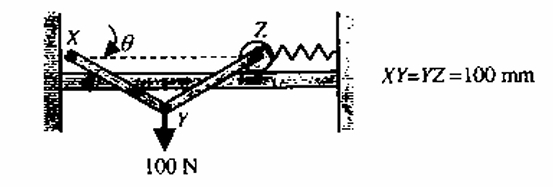
\includegraphics[width=0.6\columnwidth]{q36.png}
\caption*{}
\label{fig:q36}
\end{figure}
\hfill{\brak{\text{GATE PI 2010}}}
\begin{enumerate}
\begin{multicols}{2}
\item $\frac{5}{3}\sqrt{3}$
\item $\frac{5}{2}\sqrt{3}$
\item $5\sqrt{3}$
\item $10\sqrt{3}$
\end{multicols}
\end{enumerate}

\item A cantilever beam XY is made of a stepped circular shaft of diameters $100$ mm and $50$ mm, as shown in the following figure. The cantilever is subjected to two concentrated bending moments, one of $100$ Nm at point Y and another of $200$ Nm at point Z. The maximum bending stress \brak{\text{in MPa}} experienced by the cantilever is
\begin{figure}[h]
\centering
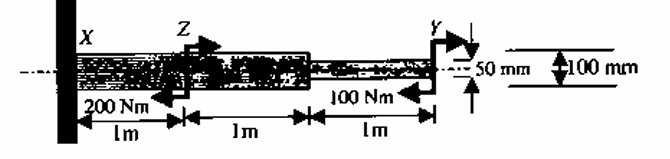
\includegraphics[width=0.8\columnwidth]{q37.png}
\caption*{}
\label{fig:q37}
\end{figure}
\hfill{\brak{\text{GATE PI 2010}}}
\begin{enumerate}
\begin{multicols}{2}
\item $1.02$
\item $3.06$
\item $8.15$
\item $16.30$
\end{multicols}
\end{enumerate}

\item A $1$ m long cylindrical shaft of diameter $100$ mm is joined to the wall by means of fillet weld as shown in the following figure. The shaft is designed to carry a torque of $5$ kNm at the free end. If the allowable shear stress of the weld material is $80$ MPa, then the minimum value of the size, L \brak{\text{shown in the following figure}}, of the fillet \brak{\text{in mm}} is
\begin{figure}[H]
\centering
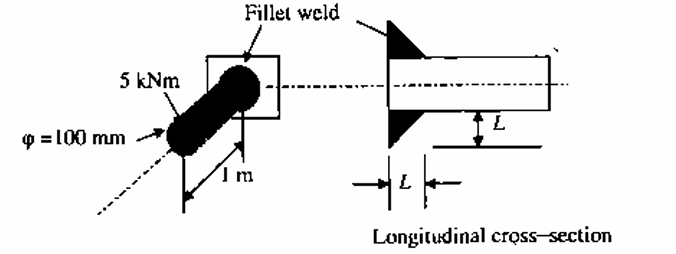
\includegraphics[width=0.8\columnwidth]{q38.png}
\caption*{}
\label{fig:q38}
\end{figure}
\hfill{\brak{\text{GATE PI 2010}}}
\begin{enumerate}
\begin{multicols}{4}
\item $3.97$
\item $5.63$
\item $7.95$
\item $11.45$
\end{multicols}
\end{enumerate}

\item In a steam power plant, the turbine power output is $1$ MW while the boiler heat input is at the rate of $2.5$ MW. The pump power input is negligibly small. In the condenser, exhaust steam from the turbine rejects heat to a steady flow of cooling water, which enters the condenser at $25^{\circ}\text{C}$ and leaves at $40^{\circ}\text{C}$. Ignore kinetic and potential energy effects for the cooling water. The specific heat of cooling water is $4 \text{ kJ/kgK}$. The required mass flow rate \brak{\text{in kg/s}} of cooling water is
\hfill{\brak{\text{GATE PI 2010}}}
\begin{enumerate}
\begin{multicols}{4}
\item $1.5$
\item $2.5$
\item $15$
\item $25$
\end{multicols}
\end{enumerate}

\item Nitrogen gas flows over a flat surface, which is maintained at a temperature \brak{T_w} of $300$ K. The temperature distribution within the boundary layer is expressed as:
$$ \frac{T - T_w}{T_{\infty} - T_w} = 1 - e^{-3500y} $$
where y \brak{\text{in m}} is the distance normal to the surface, the free stream nitrogen gas temperature \brak{T_{\infty}} is $400$ K, and T is the Nitrogen gas temperature within the boundary layer at a given y. The thermal conductivity of nitrogen is $0.03$ W/mK. The resulting average convective heat transfer coefficient \brak{\text{in $\text{W/m}^2\text{K}$}} is
\hfill{\brak{\text{GATE PI 2010}}}
\begin{enumerate}
\begin{multicols}{4}
\item $52$
\item $105$
\item $1050$
\item $3500$
\end{multicols}
\end{enumerate}

\item Consider steady and incompressible flow of water through a tapered pipe from section 1 to section 2. The pipe has a diameter of $0.25$ m and a centre-line elevation of $25$ m at section 1 and a diameter of $0.35$ m and a centre-line elevation of $20$ m at section 2. Consider head loss between section 1 and section 2 to be negligibly small. Pressure at section 1 is $120$ kPa. The acceleration due to gravity is $10 \text{ m/s}^2$ and density of water is $1000 \text{ kg/m}^3$. For a flow rate of $0.2 \text{ m}^3\text{/s}$, the pressure at section 2 \brak{in kPa} is
\hfill{\brak{\text{GATE PI 2010}}}
\begin{enumerate}
\begin{multicols}{4}
\item $56$
\item $112$
\item $176$
\item $232$
\end{multicols}
\end{enumerate}

\item If annual demand, ordering cost and carrying cost become four times of their respective original values, then the economic order quantity \brak{EOQ}
\hfill{\brak{\text{GATE PI 2010}}}
\begin{enumerate}
\begin{multicols}{4}
\item remains the same
\item gets halved
\item gets doubled
\item becomes four times
\end{multicols}
\end{enumerate}

\item The solution of the differential equation $\frac{dy}{dx} - y^2 = 1$ satisfying the condition $y\brak{0}=1$ is
\hfill{\brak{\text{GATE PI 2010}}}
\begin{enumerate}
\begin{multicols}{4}
\item $y = e^{x^2}$
\item $y = \sqrt{x}$
\item $y = \cot\brak{x + \frac{\pi}{4}}$
\item $y = \tan\brak{x + \frac{\pi}{4}}$
\end{multicols}
\end{enumerate}

\item Two white and two black balls, kept in two bins, are arranged in four ways as shown below. In each arrangement, a bin has to be chosen randomly and only one ball needs to be picked randomly from the chosen bin. Which one of the following arrangements has the highest probability for getting a white ball picked?
\hfill{\brak{\text{GATE PI 2010}}}

\begin{figure}[H]
\centering
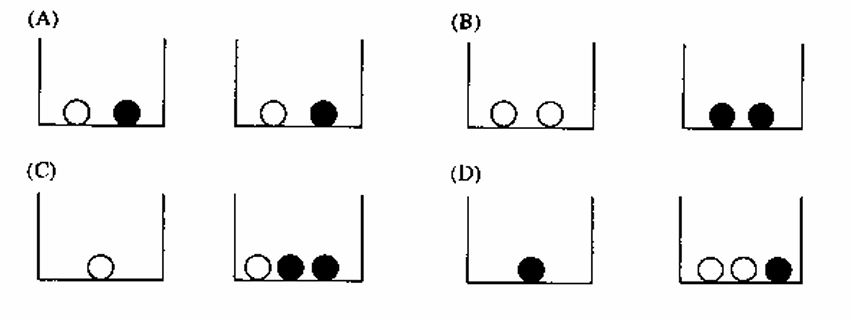
\includegraphics[width=0.8\columnwidth]{q44.png}
\caption*{}
\label{fig:q44}
\end{figure}


\item An industrial process consists of the following six activities
\begin{enumerate}
    \item[1.] Casting
    \item[2.] Wait
    \item[3.] To Buffing
    \item[4.] Buffing
    \item[5.] Inspection
    \item[6.] Store
\end{enumerate}
The correct flow process chart for this process is
\hfill{\brak{\text{GATE PI 2010}}}

\begin{figure}[H]
\centering
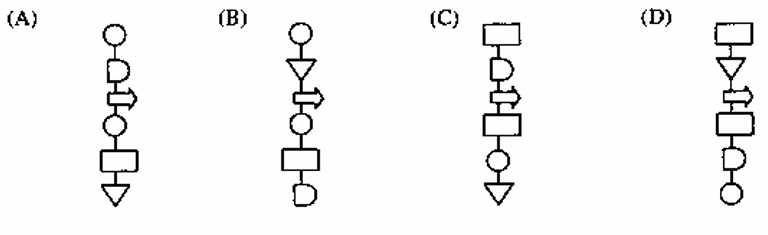
\includegraphics[width=0.6\columnwidth]{q45.png}
\caption*{}
\label{fig:q45}
\end{figure}


\item A batch of $10,000$ raw work units is processed through $20$ operations, each of which has a fraction defect rate of $0.05$. The defect-free units and the number of defects in the final batch are, respectively,
\hfill{\brak{\text{GATE PI 2010}}}
\begin{enumerate}
\begin{multicols}{4}
\item $3285$ and $6715$
\item $3385$ and $6615$
\item $3485$ and $6515$
\item $3585$ and $6415$
\end{multicols}
\end{enumerate}

\item Match the following groups most appropriately.
\begin{table}[h]
\caption*{}
\label{tab:q47}
\centering
\begin{tabular}{llcl}
\multicolumn{2}{l}{\textbf{Group I}} & \multicolumn{2}{l}{\textbf{Group II}} \\
E. & Strategic decision & 1. & Production scheduling \\
F. & Bullwhip effect & 2. & Reduce manufacturing lead time \\
G. & Flexible manufacturing system & 3. & Plant layout \\
H. & Tactical decision & 4. & Price fluctuations \\
I. & Operational decision & 5. & Inventory policies \\
\end{tabular}
\end{table}
\hfill{\brak{\text{GATE PI 2010}}}
\begin{enumerate}
\begin{multicols}{2}
\item E-3, F-4, G-2, H-5, I-1
\item E-4, F-5, G-1, H-2, I-3
\item E-4, F-1, G-5, H-3, I-2
\item E-3, F-1, G-2, H-5, I-4
\end{multicols}
\end{enumerate}
\noindent
\textbf{Common Data for Questions 48 and 49:}

\vspace{1em}

\noindent
A machine shop processes custom orders from a variety of clients. A machining centre in a job shop for a local manufacturing company has five unprocessed jobs remaining at a particular point in time. The jobs are labelled $J_1, J_2, J_3, J_4,$ and $J_5$ in the order they entered the shop. The respective processing times and due dates are given in the table below:

\vspace{1em}

\begin{center}
\begin{tabular}{|c|c|c|}
\hline
\textbf{Job} & \textbf{Processing time (in days)} & \textbf{Due date (in days)} \\
\hline
$J_1$ & 13 & 65 \\
\hline
$J_2$ & 32 & 48 \\
\hline
$J_3$ & 34 & 34 \\
\hline
$J_4$ & 4  & 36 \\
\hline
$J_5$ & 5  & 35 \\
\hline
\end{tabular}
\end{center}

\item When the jobs are assumed to enter the shop in the sequence of SPT \brak{\text{Shortest Processing Time}}, the mean flow time and average tardiness, respectively, are
\hfill{\brak{\text{GATE PI 2010}}}
\begin{enumerate}
\begin{multicols}{2}
\item $35.4$ and $12$
\item $37.4$ and $13$
\item $39.4$ and $14$
\item $41.4$ and $15$
\end{multicols}
\end{enumerate}

\item When the jobs are assumed to enter in the sequence of EDD \brak{\text{Earliest Due Date}}, the number of tardy jobs is
\hfill{\brak{\text{GATE PI 2010}}}
\begin{enumerate}
\begin{multicols}{4}
\item $0$
\item $1$
\item $3$
\item $4$
\end{multicols}
\end{enumerate}
\noindent
\textbf{Common Data for Questions 50 and 51:}

\vspace{1em} % Adds a bit of vertical space

\noindent
A company is engaged in producing and selling a single product. The fixed cost of the product is $F$ per period. The selling price for the product is $S$ per unit. The variable cost is $V$ per unit, which is half of the selling price, i.e., $S/2$ per unit. The company has computed its Break Even Sales in monetary units. Not being satisfied with this Break Even Sales, the company has decided to increase its selling price from $S$ to $1.5S$. The company has again computed the new Break Even Sales in monetary units keeping the fixed cost $\brak{F}$ and variable cost \brak{S/2\text { per unit}} of the product same.


\item The ratio of new to old Break Even Sales is
\hfill{\brak{\text{GATE PI 2010}}}
\begin{enumerate}
\begin{multicols}{4}
\item $0.25$
\item $0.50$
\item $0.75$
\item $1.50$
\end{multicols}
\end{enumerate}

\item The firm desires to make a profit equal to the fixed cost of the product. In this scenario, the ratio of new to old Required Sales Volume is
\hfill{\brak{\text{GATE PI 2010}}}
\begin{enumerate}
\begin{multicols}{4}
\item $0.25$
\item $0.50$
\item $0.75$
\item $1.50$
\end{multicols}
\end{enumerate}
\noindent 
\textbf{Linked Answer Questions}

\vspace{1em} % Adds a bit of vertical space

\noindent 
\textbf{Statement for Linked Answer Questions 52 and 53:}

\vspace{1em}

\noindent 
Consider the following Linear Programming problem:

\begin{align*}
    \text{Maximize } \quad & Z = 3x_1 + 5x_2 + 8x_3 \\
    \text{Subject to: } \quad & x_1 + 5x_2 \leq 10 \\
    & x_3 \leq 20 \\
    & x_1 \geq 0; \; x_2 \geq 0; \; x_3 \geq 0
\end{align*}

\item Apart from the non-negativity criteria, the dual problem for the given Linear Programming problem consists of
\hfill{\brak{\text{GATE PI 2010}}}
\begin{enumerate}
\item $2$ constraints and both of them are of $\le$ type
\item $2$ constraints and both of them are of $\ge$ type
\item $3$ constraints and all of them are of $\le$ type
\item $3$ constraints and all of them are of $\ge$ type
\end{enumerate}

\item The value of the objective function after solving the dual problem is
\hfill{\brak{\text{GATE PI 2010}}}
\begin{enumerate}
\begin{multicols}{4}
\item $160$
\item $170$
\item $190$
\item $210$
\end{multicols}
\end{enumerate}
\noindent 
\textbf{Statement for Linked Answer Questions 54 and 55:}

\vspace{1em} % Adds vertical space

\noindent 
In orthogonal turning of an engineering alloy, it has been observed that the friction force acting at the chip-tool interface is 402.5 N and the friction force is also perpendicular to the cutting velocity vector. The feed velocity is negligibly small with respect to the cutting velocity. The ratio of friction force to normal force associated with the chip-tool interface is 1. The uncut chip thickness is 0.2 mm and the chip thickness is 0.4 mm. The cutting velocity is 2 m/s.

\item The shear force \brak{\text{in N}} acting along the primary shear plane is
\hfill{\brak{\text{GATE PI 2010}}}
\begin{enumerate}
\begin{multicols}{4}
\item $180.0$
\item $240.0$
\item $360.5$
\item $402.5$
\end{multicols}
\end{enumerate}

\item Assume that the energy expended during machining is completely converted to heat. The rate of heat generation \brak{\text{in W}} at the primary shear plane is
\hfill{\brak{\text{GATE PI 2010}}}
\begin{enumerate}
\begin{multicols}{4}
\item $180.5$
\item $200.5$
\item $302.5$
\item $402.5$
\end{multicols}
\end{enumerate}

\item Choose the most appropriate word from the options given below to complete the following sentence:
His rather casual remarks on politics \underline{\hspace{2cm}} his lack of seriousness about the subject.
\hfill{\brak{\text{GATE GA 2010}}}
\begin{enumerate}
\begin{multicols}{2}
\item masked
\item belied
\item betrayed
\item suppressed
\end{multicols}
\end{enumerate}

\item Which of the following options is the closest in meaning to the word below:
Circuitous
\hfill{\brak{\text{GATE GA 2010}}}
\begin{enumerate}
\begin{multicols}{2}
\item cyclic
\item indirect
\item confusing
\item crooked
\end{multicols}
\end{enumerate}

\item Choose the most appropriate word from the options given below to complete the following sentence:
If we manage to \underline{\hspace{2cm}} our natural resources, we would leave a better planet for our children.
\hfill{\brak{\text{GATE GA 2010}}}
\begin{enumerate}
\begin{multicols}{2}
\item uphold
\item restrain
\item cherish
\item conserve
\end{multicols}
\end{enumerate}

\item $25$ persons are in a room. $15$ of them play hockey, $17$ of them play football and $10$ of them play both hockey and football. Then the number of persons playing neither hockey nor football is
\hfill{\brak{\text{GATE GA 2010}}}
\begin{enumerate}
\begin{multicols}{4}
\item $2$
\item $17$
\item $13$
\item $3$
\end{multicols}
\end{enumerate}

\item The question below consists of a pair of related words followed by four pairs of words. Select the pair that best expresses the relation in the original pair.
Unemployed : Worker
\hfill{\brak{\text{GATE GA 2010}}}
\begin{enumerate}
\begin{multicols}{2}
\item fallow : land
\item unaware : sleeper
\item wit : jester
\item renovated : house
\end{multicols}
\end{enumerate}

\item If $137 + 276 = 435$ how much is $731 + 672$?
\hfill{\brak{\text{GATE GA 2010}}}
\begin{enumerate}
\begin{multicols}{4}
\item $534$
\item $1403$
\item $1623$
\item $1513$
\end{multicols}
\end{enumerate}

\item Hari \brak{H}, Gita \brak{G}, Irfan \brak{I} and Saira \brak{S} are siblings \brak{\text{i.e. brothers and sisters}}. All were born on $1^{st}$ January. The age difference between any two successive siblings \brak{that is born one after another} is less than $3$ years. Given the following facts:
\begin{enumerate}
    \item[i.] Hari's age + Gita's age > Irfan's age + Saira's age.
    \item[ii.] The age difference between Gita and Saira is $1$ year. However, Gita is not the oldest and Saira is not the youngest.
    \item[iii.] There are no twins.
\end{enumerate}
In what order were they born \brak{\text{oldest first}}?
\hfill{\brak{\text{GATE GA 2010}}}
\begin{enumerate}
\begin{multicols}{4}
\item HSIG
\item SGHI
\item IGSH
\item IHSG
\end{multicols}
\end{enumerate}

\item Modern warfare has changed from large scale clashes of armies to suppression of civilian populations. Chemical agents that do their work silently appear to be suited to such warfare; and regretfully there exist people in military establishments who think that chemical agents are useful tools for their cause.
Which of the following statements best sums up the meaning of the above passage:
\hfill{\brak{\text{GATE GA 2010}}}
\begin{enumerate}
\item Modern warfare has resulted in civil strife.
\item Chemical agents are useful in modern warfare.
\item Use of chemical agents in warfare would be undesirable.
\item People in military establishments like to use chemical agents in war.
\end{enumerate}

\item $5$ skilled workers can build a wall in $20$ days; $8$ semi-skilled workers can build a wall in $25$ days; $10$ unskilled workers can build a wall in $30$ days. If a team has $2$ skilled, $6$ semi-skilled and $5$ unskilled workers, how long will it take to build the wall?
\hfill{\brak{\text{GATE GA 2010}}}
\begin{enumerate}
\begin{multicols}{4}
\item $20$ days
\item $18$ days
\item $16$ days
\item $15$ days
\end{multicols}
\end{enumerate}

\item Given digits $2, 2, 3, 3, 3, 4, 4, 4, 4$ how many distinct $4$ digit numbers greater than $3000$ can be formed?
\hfill{\brak{\text{GATE GA 2010}}}
\begin{enumerate}
\begin{multicols}{4}
\item $50$
\item $51$
\item $52$
\item $54$
\end{multicols}
\end{enumerate}

\end{enumerate}
\end{document}
